\documentclass[a4paper]{report}
% generated by Docutils <http://docutils.sourceforge.net/>
\usepackage{fixltx2e} % LaTeX patches, \textsubscript
\usepackage{cmap} % fix search and cut-and-paste in Acrobat
\usepackage{ifthen}
\usepackage[T1]{fontenc}
\usepackage[utf8]{inputenc}
\setcounter{secnumdepth}{0}

%%% Custom LaTeX preamble
% PDF Standard Fonts
\usepackage{mathptmx} % Times
\usepackage[scaled=.90]{helvet}
\usepackage{courier}
\usepackage{graphicx}

\usepackage{geometry}
\geometry{top=3cm, bottom=2.5cm, left=2cm, right=2cm}


%%% User specified packages and stylesheets

%%% Fallback definitions for Docutils-specific commands

% hyperlinks:
\ifthenelse{\isundefined{\hypersetup}}{
  \usepackage[colorlinks=true,linkcolor=blue,urlcolor=blue]{hyperref}
  \urlstyle{same} % normal text font (alternatives: tt, rm, sf)
}{}
\hypersetup{
  pdftitle={FiveBot},
}

%%% Title Data
\title{\phantomsection%
  FiveBot%
  \label{fivebot}}
\author{Thomas Lechat \and HAUM \and Mathieu Gaborit}
\date{Mai 2012}

%%% Table of contents

\setcounter{tocdepth}{4}
\renewcommand{\contentsname}{Table des matières}

%%% Body
\begin{document}
\maketitle

\tableofcontents
\newpage


\section{Objectif%
  \label{objectif}%
}

Le but des manoeuvres sur ce système était de le faire fonctionner \textbf{correctement}.
Avant d'aller plus loin, il est important de noter que c'est un parfait échec.

Dans le cadre du HackerSpace de l'Université du Maine (HAUM, une section plus ou moins informelle de l'association Asimov), nous avons pris part à un projet autour de la plateforme robotique Fivebot.

Le projet nous a été proposé, nous aurions pu le refuser.
L'idée nous a, à la base, intéressés et notre échec, s'il est cuisant, est en grande partie dû au manque de documentation.
Ni celui qui nous a fourni le projet ni même la société Génération Robots ne sont responsables de cet échec.
Notons simplement que plus de documentation aurait été nécessaire.

Le tout premier objectif était la prise en main de ladite plateforme et sa programmation basique, en particulier la création d'une couche basse permettant une interaction plus facile pour d'autres étudiants ou utilisateurs par la suite.
Le second était bien entendu de parvenir à faire fonctionner tous les capteurs (bumpers, infra-rouges et ultra-sonores) ainsi que les moteurs.
Enfin dans un second temps, il s'agissait d'approfondir avec l'exploitation du robot pour divers tests mais aussi la mise en oeuvre de systèmes d'exploration simples et l'intégration d'autres composants (caméra ip, etc...).

A noter que le présent document est publié et distribué selon les termes de la Licence Creative Commons Paternité - Partage à l'Identique 3.0 non transposé {[}\href{http://creativecommons.org/licenses/by-sa/3.0/}{LICENSE}{]}.

De leur côté, les codes implémentés par nos soins sont mis à disposition sous license GNU/GPLv3 ou supérieure.
Ils sont par ailleurs largement inspirés de ceux qui nous ont été fournis en début de projet et sur lesquels aucune licence n'était spécifiée. Ces codes originaux sont dans les fichiers commentés :

\begin{verbatim}

// J. Lehuen 2011

\end{verbatim}

et dans le fichier nommé \texttt{FB004\_Sample.pde} fourni par \href{http://www.fivebro.com.tw/}{Fivebro}.


\section{Informations générales recueillies sur le robot%
  \label{informations-generales-recueillies-sur-le-robot}%
}

Le robot est un Fivebot, de la compagnie \href{http://www.fivebro.com.tw/}{Fivebro} (d'après internet), commercialisé par \href{http://www.generationrobots.com}{Generation Robots}.

Il nous a été fourni monté, avec la documentation d'origine (orientée vers le montage), disponible en annexe. Cette documentation était constituée d'une aide au montage et d'un listing des pièces (sans beaucoup de précision ni référence).

Nous avons donc commencé par chercher de la documentation autour du robot.
Après quelques sauts, nous avons atteint \href{http://www.fivebro.com.tw/download.htm}{cette page}.

Notons qu'une partie des liens sont morts et que, dans la section dédiée au FB004 (en bas), le zip du Sample Code semble être corrompu ; pour le reste de la documentation, nous en disposions déjà.

Nous avons donc émis l'hypothèse que ce fameux Sample Code était déjà en notre possession.
Nous l'avons trouvé dans un des dossier et examiné.


\subsection{Le sample code%
  \label{le-sample-code}%
}

L'aventure du Sample Code fut particulièrement déroutante.

En ouvrant ce fichier, nous nous attendions (comme dans pour tout Sample Code) à trouver un code clair, organisé et commenté.

Nous sommes tombés de très haut en découvrant sur un fichier de 621 lignes (504 lignes de code)... sans commentaire vraiment utile passée la 25ème ligne.

Enfin, des parties importantes du code ont été neutralisées, passées en commentaire.

Pour finir, le code contient des références à un écran LCD qui n'est pas présent et dont les spécifications ne sont pas données.

Ce SampleCode est inutilisable tel quel et a donc été fragmenté et parfois légèrement modifié par J. Lehuen pour tester tour à tour des parties du robot.

Seule la partie sur les télémètre ultra-sonore n'était pas traitée séparément du Sample Code complet


\section{Travaux réalisés et état des lieux%
  \label{travaux-realises-et-etat-des-lieux}%
}

Nous allons maintenant réaliser un état des lieux du système et décrire les travaux finalement menés sur la platforme Fivebot.
Nous aborderons aussi les problème rencontrés et, finalement, pourquoi le projet a été abandonné.


\subsection{Constats%
  \label{constats}%
}

Lors d'essais avec le robot, nous avons notés plusieurs choses étranges (des erreurs de conception ?).

Aucune protection n'est assurée quand à l'inversion de la chaine motrice : forcer la rotation des moteurs revient à placer un générateur dans le circuit.
Une tension est alors appliquée aux cartes programmables, depuis les moteurs.

Même si cela ne semble pas poser de problème dans ce cas précis, il aurait pu être bon de protéger le système contre ça avec un pont en H pour l'alimentation des moteurs (ils utilisent un courant continu) et une diode de roue libre pour la protection par exemple. Cette information n'était pas présente dans la documentation et aurait été d'autant plus importante si le robot avait eu à parcourir des surfaces non planes car il aurait alors fallu gérer avec précision les descentes.

Ce qui nous a également semblé étonnant concerne l'alimentation de ces moteurs : la ``puissance'' est imposée via la fonction:
%
\begin{verbatim}

analogWrite(sortie\_moteur, puissance\_voulue);

\end{verbatim}

Cette fonction admet n'importe quel port supportant la PWM comme premier argument et un entier entre 0 et 255 comme second (on nous a signifié, en début de projet, que le robot devait être commandé entre 0 et 100).

Les fonctions PWM (pulse width modulation) fournies par l'arduino \textbf{ne générent pas} un signal continu mais bien un signal alternatif carré dont la valeur moyenne dépend de son rapport cyclique (défini par le second argument).

Dans ces conditions, que reçoit le moteur ? un signal carré ou continu ?
Si aucune transformation n'est faite sur ce signal, on se retrouve dans le premier cas.
Ce n'est pas très grave, mais nous aurions (si nous avions eu à le concevoir) au moins essayé d'isoler la partie commande et la partie puissance avec un montage suiveur de tension par exemple (à base d'amplificateur opérationnel).
Ainsi, les caractèristiques du circuit n'auraient pas été fonction du courant demandé et la tension imposée.


\subsection{Travail Mené%
  \label{travail-mene}%
}

Note 1: Aucune indication technique \emph{fiable} n'était fournie sur les éléments clés de l'architecture. Les seules informations que nous ayons sont issues des codes sources fournis et de tests.
Note 2: La carte programmable n'est pas clairement identifiée. Elle est sérigraphiée ``EDVACArduino'' ce qui n'a malheureusement aidé en rien.


\subsubsection{Bumpers%
  \label{bumpers}%
}

Les bumpers sont les premiers éléments auxquels nous nous sommes intéressés.
Rien de bien compliqué ici, même si le fait que ceux ci ne soient pas reliés à une interruption est grandement discutable.

A la décharge du concepteur, le microcontrôleur choisi ne dispose que de 2 interruptions alors qu'il en aurait fallu au moins 3 (si on réunit les 3 bumpers sous une seule interruption, les deux autres servant aux roues codeuses).

Malgré cela, les bumpers fonctionnent parfaitement : ils étaient, pour nous, reliés aux pins 8, 9 et 10.
La détection fonctionne sans problème, mais nécessite un contrôle régulier type \emph{polling loop} (vérification régulière par une boucle).

Le code produit pour simplifier l'utilisation est le suivant:

\begin{verbatim}
#ifndef bumpers_h
#define bumpers_h

// This pins are freely modifiable arccording to your
// mapping on the bot.
#define BOT_RIGHTBUMPER 10 // Bumper right --> pin8
#define BOT_MIDDLEBUMPER 9 // Bumper middle --> pin9
#define BOT_LEFTBUMPER 8 // Bumper left --> pin10

// This macro returns true if a bumpers has been hit. False else.
#define getBumperState(bumper_pin) (!digitalRead(bumper_pin))

// True if something hit one of the bumpers
#define getCollision (BOT_getBumperState(BOT_LEFTBUMPER) ||
        BOT_getBumperState(BOT_MIDDLEBUMPER) ||
        BOT_getBumperState(BOT_RIGHTBUMPER))

// This initialize bumpers.
// Just remind to add that in your setup().
// The only thing it does is pinMode each bumper pin as INPUT
void _init_bumpers();

void _init_bumpers() {
    pinMode(BOT_LEFTBUMPER, INPUT);
    pinMode(BOT_MIDDLEBUMPER, INPUT);
    pinMode(BOT_MIDDLEBUMPER, INPUT);
}

#endif
\end{verbatim}

Ce code permet des boucles simples pour la vérification

\begin{verbatim}
while(1) { // coutume de la boucle infinie en systèmes automatisés
    while(!getCollision) {
        // ... faire avancer le robot
    }

    // stoper le robot
    // modifier la trajectoire ou autre
} // retour à la boucle
\end{verbatim}

Les bumpers sont donc parfaitement opérationnels et les fonctions associées sont implémentées.


\subsubsection{Capteurs Infra-rouges%
  \label{capteurs-infra-rouges}%
}

L'utilisation des capteurs infrarouges proposée dans les codes fournis est particulièrement étonnante

\begin{verbatim}
int ir_distance(unsigned char ir)
{
    int val = analogRead(ir);
    return (6762/(val-9))-4;
}
\end{verbatim}

Notons que cette fonction est identique à celle proposée ligne 226 du Sample Code Fivebro.

Rien dans la documentation ne nous indique d'où viennent ces coefficients.
Rien non plus n'identifie les capteurs (référence, datasheet, etc...).

Fatigués de devoir jouer contre la logique, nous avons admis que cette formule était bonne et l'avons testée : même si elle renvoie des résultats cohérents, ceux ci sont loin d'être suffisants pour une utilisation précise.

Finalement, nous avons fait plusieurs tests avec des valeurs plus ``rationnelles'' des coefficients, tests qui n'ont absolument rien donné.
Là encore, le cruel manque de documentation sur le schéma de câblage de ces capteurs nous a bloqué : comment savoir si l'information est pré-conditionnée ? comment déterminer la nature de ce conditionnement s'il existe ?
La carte utilisée n'étant pas une arduino \emph{``normale''}, pas moyen de savoir \textbf{simplement} si les entrées sont filtrées/conditionnées...

Le code produit par rapport à ces capteurs se base sur celui fourni, faute d'informations

\begin{verbatim}
#ifndef INFRARED_H_INCLUDED
#define INFRARED_H_INCLUDED

// Constants for processing
#define N_AVERAGE  3  // Number of tests over IR
#define BOT_TIME_BETWEEN 25// Time between 2 tests

// Constants for IR sensors
#define BOT_IRG 0
#define BOT_IRC 1
#define BOT_IRD 2

int BOT_getDistance(int sensor) {
    return (6762/(analogRead(sensor)-9))-4;
}

float BOT_getDistAverage(int sensor){
    int i;
    float sum = 0;
    for (i = 0; i < N_AVERAGE; i++) {
        sum += getDistance(sensor);
        delay(TIME_BETWEEN);
    }
    return sum/N_AVERAGE;
}

#endif // INFRARED_H_INCLUDED
\end{verbatim}

L'implémentation comprend une fonction pour la récupération de la distance (via la formule étrange donnée plus haut) et une seconde pour faire une moyenne sur 3 mesures. Les constantes \texttt{N\_AVERAGE} et \texttt{BOT\_TIME\_BETWEEN} permettent de paramètrer la seconde fonction en choisissant le nombre de mesures à moyenner et le temps entre chaque mesure.

Pour être efficace, cette fonction suggère que le robot soit à l'arrêt.

Nous aurions aussi pu implémenter une fonction permettant de calculer la vitesse d'approche d'un obstacle (via la dérivée de la distance par rapport au temps).

Les capteurs infrarouges sont donc opérationnels même si on constante une fluctuation d'environ 4 a 5 centimètres sur les mesures ce qui est nettement insuffisant pour calculer des trajectoires précises mais peut éventuellement permettre une détection d'obstacle (avec toujours l'inconvénient de l'absence d'interruptions...).


\subsubsection{Télémètres ultrasonores%
  \label{telemetres-ultrasonores}%
}

Les télémètres ont été notre plus grande déception.

La documentation ne donne pas de référence, ce qui, déjà, est un mauvais point.

La seule chose que nous savons est qu'ils utilisent une liaison RS485 pour la connexion avec les cartes programmables.
Celle ci est apparement à activer via 3 shunts à placer sur l'I/O Expansion Board. La documentation suggère une position sans pour autant être claire : en effet, la mise en place des shunts empêche l'upload de programmes vers la carte : on pense donc que les capteurs se connectent via une liaison série qui prend la place de celle utilisée par l'ordinateur.

Après quelques recherches, nous avons eu la confirmation que la norme RS485 n'était pas une norme logicielle mais matérielle.

Seul document en notre possession pour le détail du protocole utilisé : le fichier \texttt{URM04 Manual.pdf}

Celui-ci donne les commandes à envoyer et les réponses possibles pour deux types de capteurs : ultra-sonores et température/hygrométrie.

Le Sample Code implémente une connexion avec ces capteurs via les fonctions nommées \texttt{urm*}.
Il faut noter que même la connexion proposée par le sample code n'a jamais fonctionné sur ce robot et que, même en tentant des connexions, nous n'avons jamais obtenu de réponse des capteurs.

Nous émettons l'hypothèse que d'autres manipulations sont a faire pour activer cette connexion, celles ci n'étant pas détaillées.


\subsection{Roues codeuses%
  \label{roues-codeuses}%
}

En examinant le robot, nous avons décelé des numéros de série ou des références de gravées sur les moteurs.
Celles ci mènent à des datasheets de groupes moteur+réducteur+roues codeuses.
Malheureusement aucune de ces datasheets ne semble être vraiment la bonne.
Nous partons une fois de plus de zéro.

Nous avons décidé de mener une série de mesures pour déterminer la résolution de la roue codeuse.
Nous avons utilisé un code permettant de compter le nombre de ticks via une liaison série et chronomètre

\begin{verbatim}
// A partir d'un code de J. Lehuen 2011

unsigned char PMG = 5; // Puissance moteur gauche --> pin5
unsigned char SMG = 4; // Sens moteur gauche --> pin4

volatile int encoderpos = 0; // Compteur de la roue codeuse
volatile int rpmcount = 0; // Compteur par itération

unsigned int rpm = 0; // Vitesse de la roue
unsigned long oldTime = 0;

void setup()
{
    Serial.begin (38400);

    pinMode(PMG,OUTPUT);
    pinMode(SMG,OUTPUT);

    attachInterrupt(INT1, interrupt, RISING);

    analogWrite(PMG, 15);
    digitalWrite(SMG, HIGH);
}

void loop()
{
    Serial.println(encoderpos, DEC);
}

void interrupt()
{
    encoderpos++;
}
\end{verbatim}

(il s'agit d'une modification du fichier test3\_encoders.pde permettant de lire le nombre de ticks, et seulement ça).

Les roues ont été marquées afin d'avoir une mesure du nombre de ticks pour un tour de roue et ce le plus précisement possible (sans matériel).
Nous avons ensuite réalisé plusieurs mesures afin de les moyenner.
Le résultat a été plutot surprenant: pour un tour de roue du robot l'arduino enregistre environ 770 ticks de la roue codeuse.
Nous en avons déduit que la roue codeuse ne se trouvait pas sur l'axe de la roue mais sur l'axe moteur avant le réducteur permettant d'augmenter le couple.
Cela peut poser un problème lors de la programmation à proprement parler.
En effet tous les programmes qui nous ont été fournis lançaient un algorithme PID simplifié à chaque tick d'une des roues (avec seulement un rapport de proportionnalité et en équilibrant une des roues par rapport à l'autre).
Cela marche relativement bien dans le cas d'un PID simplifié, mais pourrait poser problème si la gestion de la trajectoire est plus complexe car, dans ce cas, la vitesse d'exécution de l'arduino pourrait ne pas étre suffisante (\emph{a fortiori} si le robot doit effectuer d'autres tâches en ``même temps'', ce qui a été envisagé dans des utilisations ultérieures du robot).
La gestion de la trajectoire doit donc être implémentée de manière à être la plus légère possible afin de prévoir des projets ultérieurs.

Un autre problème qui s'est posé est aussi celui de la fiabilité relative des roues.
En effet on constate qu'il y a un léger jeu entre l'axe et les roues, cela peut poser problème lors du démarage notament.
Si un jeu existe et qu'il diffère pour chaque roue la trajectoire du robot pourrait être légèrement modifiée au moment de la mise en marche des moteurs et donc suivre une trajectoire pseudo-rectiligne avec un angle d'erreur par rapport à la trajectoire prévue. C'est une des hypothèses que nous avons envisagé pour expliquer les problèmes de trajectoire liés au programme de test fourni.


\section{Le problème majeur du calcul de la trajectoire du robot%
  \label{le-probleme-majeur-du-calcul-de-la-trajectoire-du-robot}%
}

Voici la fonction qui gère l'équilibrage des roues qui était fournie au début du projet

\begin{verbatim}
void pulses_balance() 
{ 
    pulses_delta = speed_right + pulses_right - pulses_left; 
    if (pulses_delta <= MINSPEED) speed_left = MINSPEED; 
    else if (pulses_delta >= MAXSPEED) speed_left = MAXSPEED; 
    else speed_left = pulses_delta; 
    advance(speed_left, speed_right); 
} 
\end{verbatim}

On constate tout d'abord que c'est un équilibrage plutot élémentaire dans le sens ou il ne suit pas d'algorithme plus classique dans le genre tel qu'un PID. On constate aussi que le code n'est pas d'une clareté transcendante, encore maintenant la logique qui a mené à sa création nous parait obscure.

Nous avons donc décidé d'écrire un PID à partir du code fourni (disponible en annexe) en implémentant, dans un premier temps, uniquement la correction en proportionnalité. Nous sommes arrivés à des trajectoires quasiment rectilignes cependant des erreurs d'origine inconnue survenaient parfois. Nous avons alors émis l'hypothèse que le problème venait du fait que nous n'avions pas de valeur de référence auxquelles comparer le nombre de ticks sur chaque roue. Dans les codes fournis ou dans ceux que nous avions réalisés jusque là une des roues était considérée comme parfaite et l'autre était corrigée en conséquence or rien ne nous prouvait que les 2 roues avaient le comportement voulu.

C'est cette constatation qui nous a amené à mesurer le nombre de ticks par tours de roue afin d'en déduire le nombre de ticks théorique pour une vitesse donnée.

Nous avons aussi chercher à déterminer la vitesse des roues soumises une commande donnée.
Nous avons réalisé une mesure de temps au tour pour des vitesses commandées de 10 à 100 (plus la valeur à 15).

Cette expérience a été réalisée le plus strictement possible, nous avons chronométré le temps mis pour une roue à faire 10 tours pour une vitesse donnée et ce plusieurs fois de suite afin de moyenner les résultats.
Le robot a été surelevé afin que les roues tournent à vide pendant les mesures.
Le code utilisé était le celui utilisé lors de la caractérisation des roues codeuses.

Les mesures réalisées ont été présentées sur un graphe pour mieux se rendre compte du problème (en bleu).
En rouge, un modèle simpliste proposé.
Il s'agit en fait d'une suite de régressions linéaires sur des pans de la courbe.
A chaque point ou le modèle propose 2 valeurs, seule la plus haute est à retenir.
On notera que le modèle proposé est toujours compris dans les 20\% d'erreur de mesures fixés.
\begin{center}
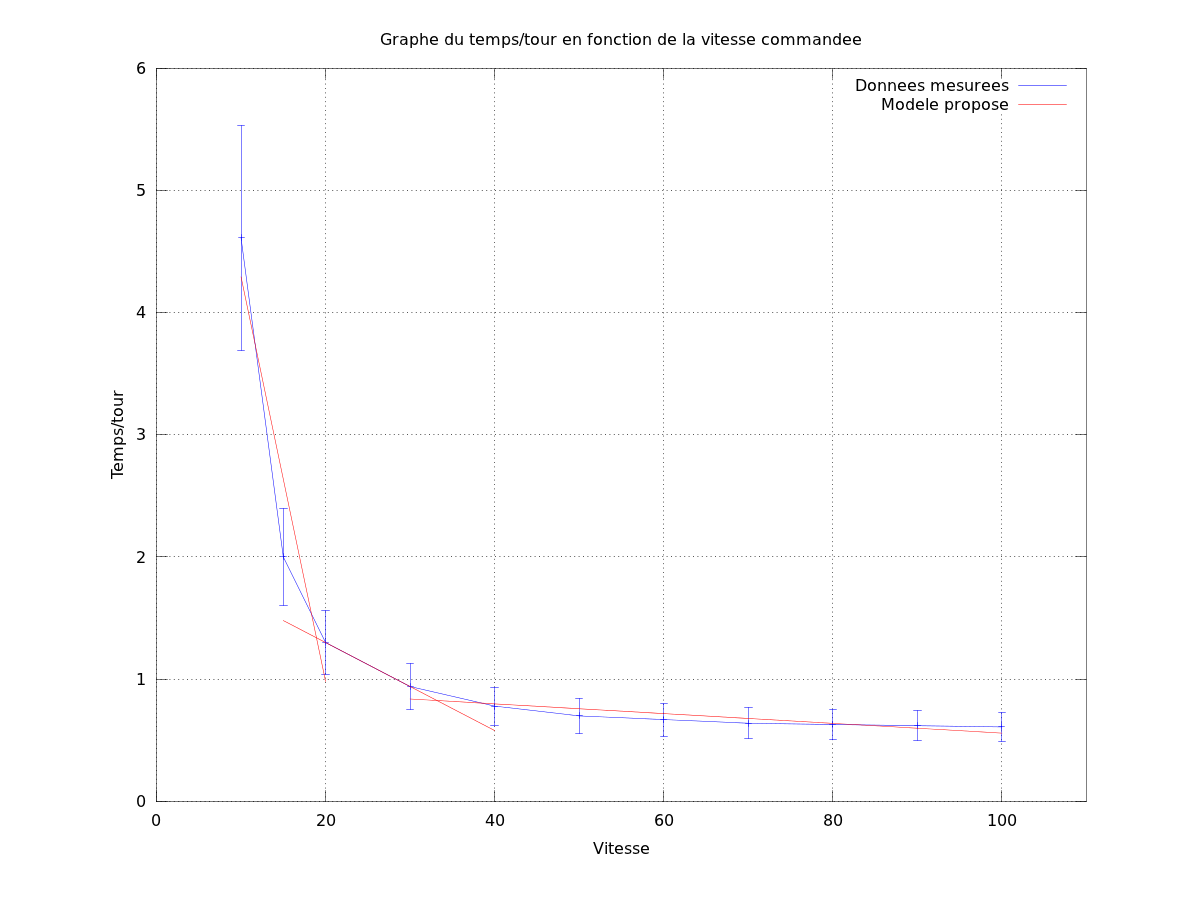
\includegraphics[width=17cm]{annexes/roues/fivebot.png}
\end{center}

Le code utilisé pour obtenir ce graphe est le suivant (sous octave):

\begin{verbatim}
clear all;
close all;

% Récupération des données
raw = load("test_bot.data")
vitesses = raw(:,1);
temps = raw(:,2);

% Incertitude de 10%
delta = 0.2*temps;

% Tracé
errorbar(vitesses, temps, delta);

% Rendre la courbe bien visible (décalage sur les axes)
xlim([0 110]);
ylim([0 6]);

% grille
grid on;

% annotations
xlabel("Vitesse");
ylabel("Temps/tour");
title("Graphe du temps/tour en fonction de la vitesse commandee");
\end{verbatim}

Le fichier \texttt{test\_bot.data} contient les données relevées suivantes :
%
\begin{verbatim}

10 4.61
15 2
20 1.3
30 0.94
40 0.78
50 0.7
60 0.67
70 0.64
80 0.63
90 0.62
100 0.61

\end{verbatim}

La première colone étant le relevé de la vitesse commandée et la seconde celui du temps au tour.

Ce graphe met largement en évidence la non-linéarité du système.
En d'autres termes la tension d'alimentation des moteurs n'est pas proportionnelle à la vitesse de rotation de ceux ci (on fait ici l'hypothèse, peut-être présomptueuse, que les moteurs sont câblés de la même manière et donc qu'ils ont les mêmes caractéristiques).
De telles mesures semblent aberrantes si on considère que les moteurs utilisés sont à courant continu ce qui d'après les documents mis à notre disposition est le cas (la réponse tension/vitesse d'un moteur CC est normalement presque rectiligne pour une charge constante).
Les mesures ne sont pas d'une grande précision du fait du protocole de mesure (un tachymètre aurait été le bienvenu plutot qu'une montre servant de chronomètre).
Cependant l'imprécision des mesures ne peut pas expliquer à elle seule la non linéarité du système, même en rajoutant des barres d'erreurs sur la courbe (ce qui est le cas en bleu ici) on voit nettement un modèle proche d'une exponentielle ou d'une fonction inverse.

Le problème d'un tel modèle est qu'il est beaucoup plus lourd et complexe à gérer.

\newpage
\section{Conclusion%
  \label{conclusion}%
}

Le système semble être relativement cohérent.
On a un système qui pose problème par le manque de documentation.

En fait, la partie motrice en particulier demanderait des modifications.
Tout d'abord, dans l'optique d'une rectification logicielle du comportement des roues (sans toucher au matériel), il faudrait prendre des mesures pour chaque vitesse et chaque roue en conditions réelles.
De ces mesures, on pourrait alors tirer un modèle de réponse pour chacune des roues et donc une fonction de la vitesse permettant de pondérer un PID.

Cette approche a le gros désavantage de demander beaucoup de mesures.

Un autre problème est la faible capacité d'une carte arduino.

En effet, lancer un calcul de pondération pour chaque roue à chaque tick d'horloge, est quelque chose de relativement lourd (très lourd pour un ATMega328, le micro-contrôleur équipant la carte).
Ensuite, ce calcul demande un certain temps, et l'arduino, ne disposant pas de parallèlisme, ne peut se permettre un si long temps dédié à une seule tâche.

On aurait pu envisager d'utiliser une implémentation paralellisée des programmes via \href{http://www.ceu-lang.org/}{Céu} par exemple ou bien d'optimiser drastiquement le code via une ré-écriture en C ARM ou ASM.
Ces solutions présentent toutefois plus de difficultées que de bénéfices.

Un autre moyen aurait été d'utiliser un réseau de cartes (au moins deux) dont une aurait été dédiée au calcul du PID (voir graphique) ou même de déporter le calcul vers un autre système.

\begin{center}
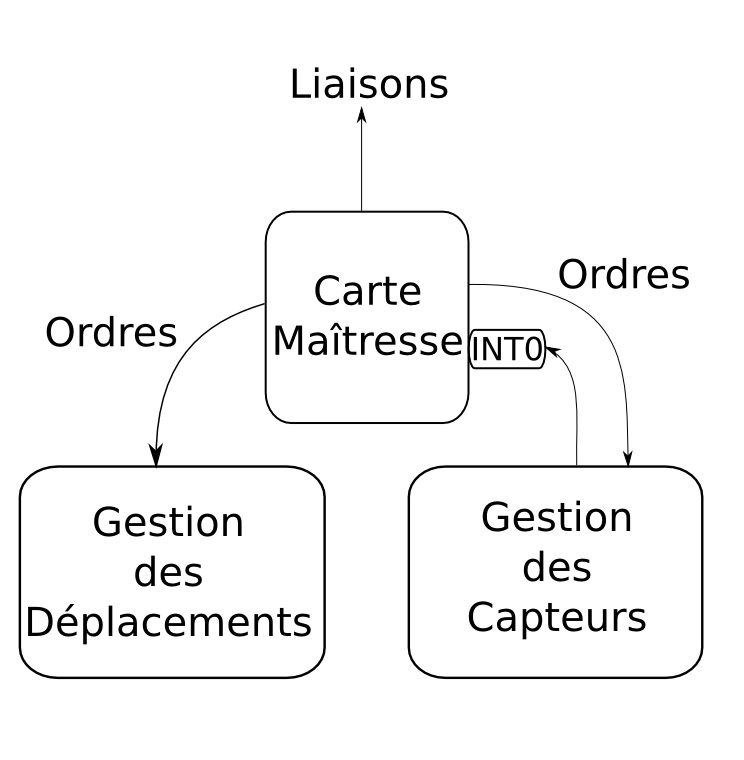
\includegraphics[width=12cm]{annexes/proposition.png}

Système multi-cartes envisageable

\end{center}

D'un point de vue plus personnel, le projet nous a d'abord beaucoup intéressé. Toutefois, passés les premiers tests et au regard de la documentation fournie, nous avons déchanté. Les dernières mesures ont mis fin au peu de motivation ayant survécu à l'absence de réponse de Génération Robots (qui s'étaient engagés à nous fournir de l'aide).

Ce projet nous a appris des choses, et, en cela, l'échec n'est pas total. L'objectif n'a toutefois pas été atteint et le nombre d'heures à passer sur le système est beaucoup trop important pour que cela soit vraiment rentable.

\newpage
\section*{Annexes%
  \label{annexes}%
}

Un dépot complet du projet est disponible ici : \url{https://github.com/haum/fivebot}

Parmi les fichiers sources du dépôt, les suivants ont été cités :
%
\begin{itemize}

\item Sample Code : \url{https://github.com/haum/fivebot/blob/master/tests/FB004_Sample.pde}

\item Bumpers (code produit) : \url{https://github.com/haum/fivebot/blob/master/lib/bumpers/bumpers.h}

\item Infra-rouges (code produit) : \url{https://github.com/haum/fivebot/blob/master/lib/infrared/infrared.h}

\item Bumpers (code fourni) : \url{https://github.com/haum/fivebot/blob/master/tests/test1_bumpers/test1_bumpers.pde}

\item Infra-Rouges (code fourni) : \url{https://github.com/haum/fivebot/blob/master/tests/test2_infrared/test2_infrared.pde}

\item Moteurs (code fourni) : \url{https://github.com/haum/fivebot/blob/master/tests/test4_motors/test4_motors.pde}

\item Roues codeuses (code fourni) : \url{https://github.com/haum/fivebot/blob/master/tests/test3_encoders/test3_encoders.pde}

\end{itemize}

Ce code nous a été fourni pour l'équilibration des roues

\begin{verbatim}
// Robot FB-004 
// Synchronisation des moteurs 
// J. Lehuen 2011 

#define MINSPEED 0 
#define MAXSPEED 100 
#define SPEED    50 

#define UNKNOWN 0 
#define ADVANCE 1 

int state = UNKNOWN; 

unsigned char PMG = 5; // Puissance moteur gauche --> pin5 
unsigned char PMD = 6; // Puissance moteur droit --> pin6 
unsigned char SMG = 4; // Sens moteur gauche --> pin4 
unsigned char SMD = 7; // Sens moteur droit --> pin7 

volatile unsigned char speed_left; 
volatile unsigned char speed_right; 
volatile unsigned long pulses_left; 
volatile unsigned long pulses_right; 
volatile int pulses_delta; 

void pulses_init() 
{ 
    pulses_left = 0; 
    pulses_right = 0; 
} 

void pulses_left_balance() 
{ 
    ++pulses_left; 
    pulses_balance(); 
} 

void pulses_right_balance() 
{ 
    ++pulses_right; 
    pulses_balance(); 
} 

void pulses_balance() 
{ 
    pulses_delta = speed_right + pulses_right - pulses_left; 
    if (pulses_delta <= MINSPEED) speed_left = MINSPEED; 
    else if (pulses_delta >= MAXSPEED) speed_left = MAXSPEED; 
    else speed_left = pulses_delta; 
    advance(speed_left, speed_right); 
} 

void init_balance(unsigned char left, unsigned char right) 
{ 
    speed_left = left; 
    speed_right = right; 
    noInterrupts(); 
    pulses_init(); 
    interrupts(); 
} 

void advance_balance(unsigned char left, unsigned char right) 
{ 
    if (state == ADVANCE) return; 
    state = ADVANCE; 
    init_balance(left, right); 
    advance(speed_left, speed_right); 
} 

void advance(unsigned char left, unsigned char right) 
{ 
    analogWrite(PMG, left); 
    digitalWrite(SMG, HIGH); 
    analogWrite(PMD, right); 
    digitalWrite(SMD, HIGH); 
} 

void setup() 
{ 
    pinMode(PMG,OUTPUT); 
    pinMode(PMD,OUTPUT); 
    pinMode(SMG,OUTPUT); 
    pinMode(SMD,OUTPUT); 

    attachInterrupt(1, pulses_left_balance, RISING); 
    attachInterrupt(0, pulses_right_balance, RISING); 
} 

void loop() 
{ 
    advance_balance(SPEED, SPEED); 
    delay(100); 
} 

\end{verbatim}

\end{document}
